%Talk given virtually for Dagstuhl 2021
\documentclass[11pt,compress,xcolor={usenames,dvipsnames},aspectratio=169]{beamer}
%\documentclass[xcolor={usenames,dvipsnames},aspectratio=169]{beamer} %slides and 
%notes
\usepackage{amsmath,
	amssymb,
	datetime,
	mathtools,
	bbm,
	%mathabx,
	array,
	booktabs,
	xspace,
	multirow,
	calc,
	colortbl,
	siunitx,
	soul,
 	graphicx}
\usepackage[usenames]{xcolor}
\usepackage[giveninits=false,backend=biber,style=nature, maxcitenames =10, mincitenames=9,mincrossrefs=10]{biblatex}
\addbibresource{FJHown23.bib}
\addbibresource{FJH23.bib}
\usepackage{newpxtext}
\usepackage[euler-digits,euler-hat-accent]{eulervm}
%\usepackage{media9}
%\usepackage[autolinebreaks]{mcode}
\usepackage[tikz]{mdframed}
\usepackage{multicol}

\usepackage{listings}
\definecolor{darkgreen}{rgb}{0,0.6,0}
\lstdefinestyle{Python}{
	%xleftmargin = -1.7in,
	showstringspaces=false,
	language        = Python,
	basicstyle      = \small\ttfamily,
	morekeywords = {as},
	keywordstyle    = \color{blue},
	stringstyle     = \color{darkgreen},
	commentstyle    = \color{darkgreen}\ttfamily,
	breaklines = true,
	postbreak=\text{$\hookrightarrow$\space},
	% style >>> and ... 
	%   see: https://tex.stackexchange.com/questions/326655/make-a-keyword-in-listings-enviorment
	alsoletter = {>,.} ,
	morekeywords = [2]{>>>,...},
	keywordstyle = [2]\color{cyan}\bfseries}


\usetheme{FJHSlimNoFoot169}
\setlength{\parskip}{2ex}
\setlength{\arraycolsep}{0.5ex}

\input FJHDef.tex

\DeclareMathOperator{\sol}{SOL}
\DeclareMathOperator{\app}{APP}
\DeclareMathOperator{\alg}{ALG}
\DeclareMathOperator{\ACQ}{ACQ}
\DeclareMathOperator{\ERR}{err}
\DeclareMathOperator{\COST}{COST}
\DeclareMathOperator{\COMP}{COMP}
\newcommand{\dataN}{\bigl(\hf(\vk_i)\bigr)_{i=1}^n}
\newcommand{\dataNj}{\bigl(\hf(\vk_i)\bigr)_{i=1}^{n_j}}
\newcommand{\dataNjd}{\bigl(\hf(\vk_i)\bigr)_{i=1}^{n_{j^\dagger}}}
\newcommand{\ERRN}{\ERR\bigl(\dataN,n\bigr)}

\newcommand{\Sapp}{S_{\textup{app}}}
\newcommand{\LambdaStd}{\Lambda^{\textup{std}}}
\newcommand{\LambdaSer}{\Lambda^{\textup{ser}}}
\newcommand{\LambdaAll}{\Lambda^{\textup{all}}}
\newcommand{\oton}{1\!:\!n}
\newcommand{\talert}[1]{\alert{\text{#1}}}
\DeclareMathOperator{\init}{init}
\DeclareMathOperator{\GP}{\cg\cp}
\newcommand{\MLE}{\textup{EB}}
\newcommand{\mCtheta}{{\mathsf{C}_{\vtheta}}}
\newcommand{\mCInv}{\mathsf{C}^{-1}}
\renewcommand{\ty}{\widetilde{y}}
\renewcommand{\tvy}{\widetilde{\vy}}

%\DeclareMathOperator{\app}{app}

\providecommand{\HickernellFJ}{H.\xspace}


\iffalse
Bayesian cubature proceeds by constructing  credible intervals for the integral based on a prior distribution for the integrand combined with sampled integrand values.  We explain this approach has been developed using low discrepancy (digital net and lattice) sampling and matching covariance kernels to expedite the computation to be much faster than $\Order(n^3)$, where $n$ is the sample size.  We tune the hyper-parameters of our covariance kernels using function data to increase the chance that the integrand is not an outlier. We also show how we have implemented these Bayesian cubature algorithms in QMCPy, a community supported Python library for quasi-Monte Carlo calculations.  Some preliminary results also call into question the Bayesian assumption.  This matter requires further study.
\fi

\renewcommand{\OffTitleLength}{-7ex}
\setlength{\FJHThankYouMessageOffset}{-8ex}
\title{Bayesian Cubature with Low Discrepancy Sequences in QMCPy}
\author[]{Fred J. Hickernell, Jagadeeswaran Rathinavel, \& Aleksei Sorokin}
\institute{Department of Applied Mathematics \qquad
	Center for Interdisciplinary Scientific Computation \\  Illinois Institute of Technology \quad
	\href{mailto:hickernell@iit.edu}{\url{hickernell@iit.edu}} \quad
	\href{http://mypages.iit.edu/~hickernell}{\url{mypages.iit.edu/~hickernell}}}

\thanksnote{Thanks to the GAIL and QMCPy teams \\
	Thanks to the organizers, especially during these unusual times \\
	Disclosure: I am multicultural (computational mathematician \& statistician)\\[2ex]
	Slides at  \href{https://speakerdeck.com/fjhickernell/dagstuhl-bayesian-cubature-ld-qmcpy}{\nolinkurl{speakerdeck.com/fjhickernell/dagstuhl-bayesian-cubature-ld-qmcpy}}}

\event{Probabilistic Numerics @ Dagstuhl}
\date[]{October 27, 2021}




\newlength{\figwidth}
\setlength{\figwidth}{0.25\textwidth}

\newlength{\figwidthSmall}
\setlength{\figwidthSmall}{0.2\textwidth}


\begin{document}
	\everymath{\displaystyle}

\frame{\titlepage}

\section{Introduction}

\begin{frame}{Our take on Bayesian \st{Quadrature} Cubature \cite{HicJag18b,RatHic19a,Jag19a,JagHic22a}}
	
	\vspace{-5ex}
		\[
	\mu :=  \int_{[0,1]^d} f(\vx) \, \dif \vx = ? \qquad \hmu_n = \text{function of } f(\vx_1),  \ldots, f(\vx_n) \qquad \text{Want } \Prob[\abs{\mu - \mu_n} \le \varepsilon] = 99\% 
	\]
	
	\begin{itemize}
		\item Assume we are \alert<1>{handed} $f \sim \GP(m,s^2 C_\vtheta)$
		\item<3-> \alert<3>{Choose $C_\vtheta$ and $\vx_1, \vx_2, \ldots$ for a \emph{fast} eigenvector-eigenvalue decomposition of the Gram matrix $\mC_\vtheta = \bigl(C_\vtheta(\vx_i, \vx_j)\bigr)_{i,j=1}^n$}; this is a \alert<3>{practical} choice, rather than informed by $f$  (see also Kanagawa, Sh\"afer, Wenger)
		\item \alert<1>{Sample} $f$ at $\vx_1, \ldots, \vx_n$
		\item<2-> \alert<2>{Tune the hyperparameters by empirical Bayes so that $f$ is not an \emph{outlier}}
		\item Construct a \alert<1>{credible interval} for $\mu$ in terms of the posterior mean $\hmu_n$
		\item \alert<1>{Increase $n$} until the half-width is no greater than $\varepsilon$
		\item<4-> \alert<4>{Implement in software:  GAIL \cite{ChoEtal21a} and QMCPy \cite{QMCPy2020a}} (see also Naslidynk, Pleiss, ProbNum)
	\end{itemize}
	
\end{frame}

\section{Matched Data Sites \& Covariance Kernels}

\begin{frame}{Low Discrepancy (LD) Sequences for Quasi-Monte Carlo (QMC) Methods}
	
\vspace{-3ex}
	
\only<1>{IID sequences have \alert{clusters and gaps}
	
	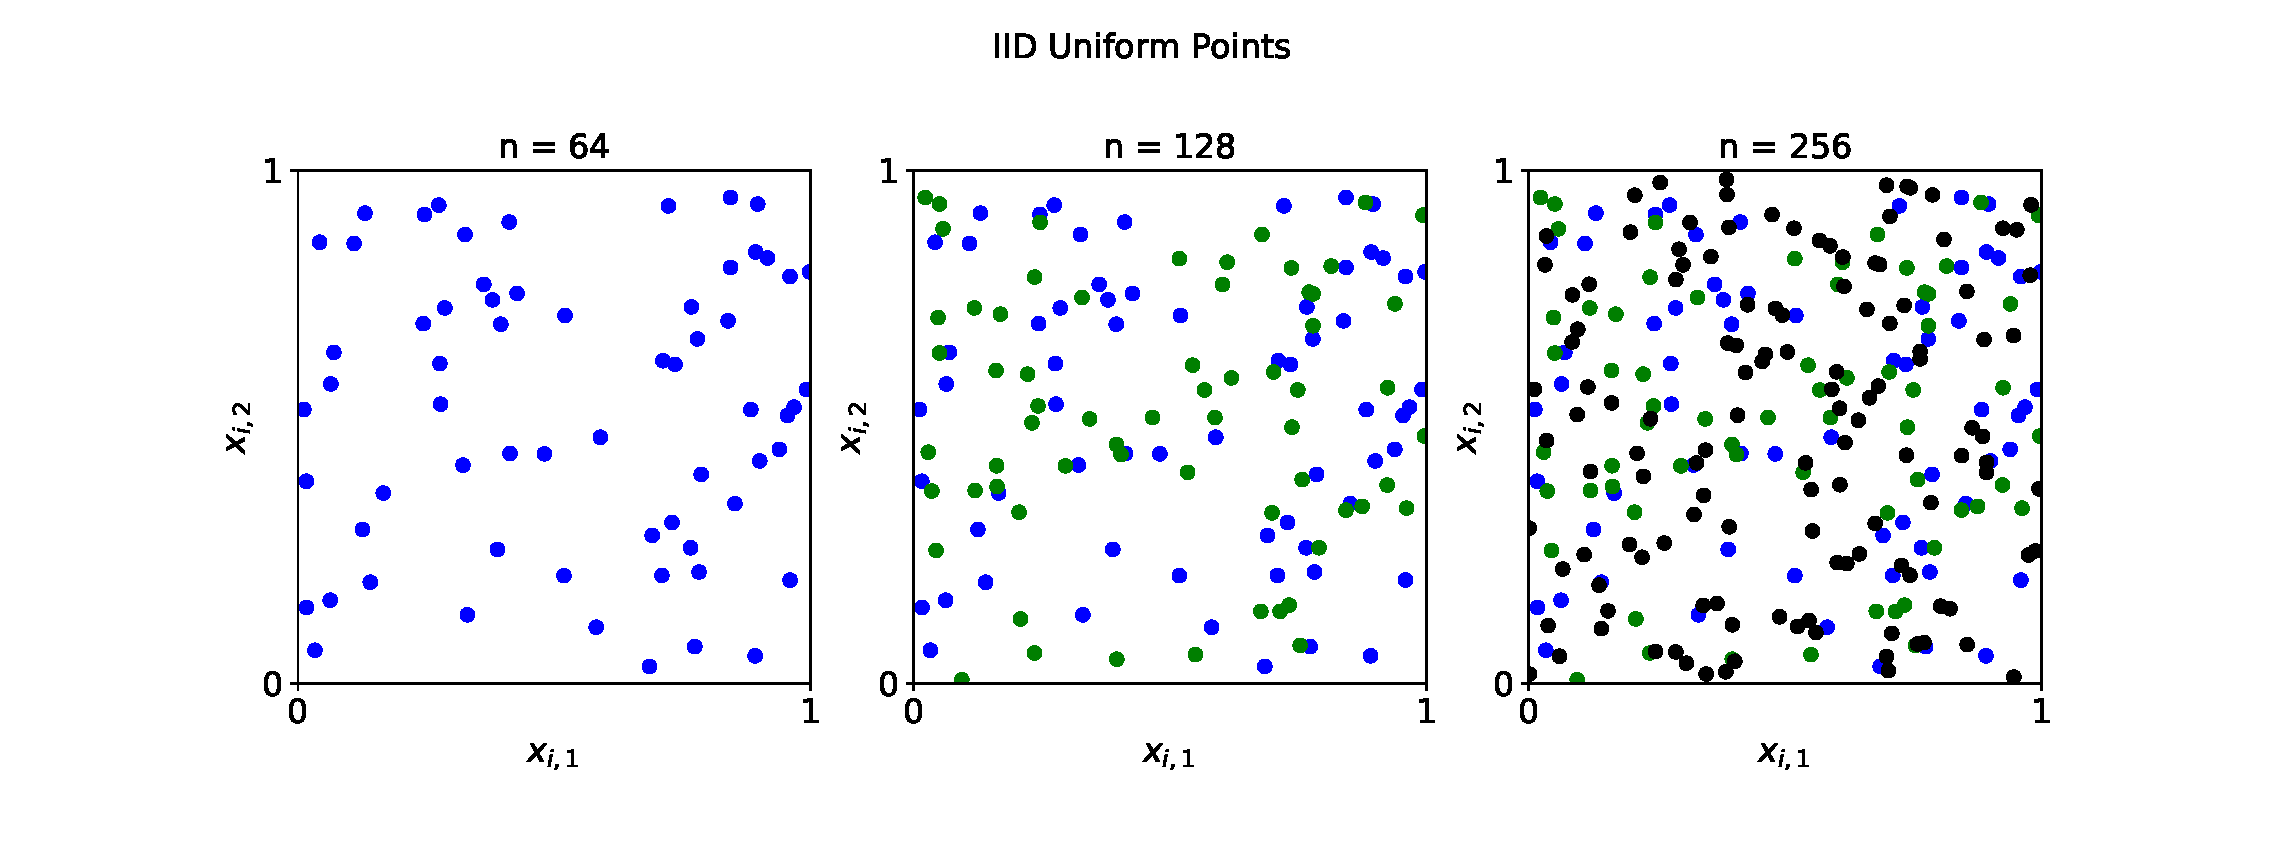
\includegraphics[width = \textwidth]{figures/dd_IID_Uniform.eps}
}
\only<2>{LD lattice sequences \cite{SloJoe94,Lem09a,DicEtal14a} are more even than IID and give faster convergence
	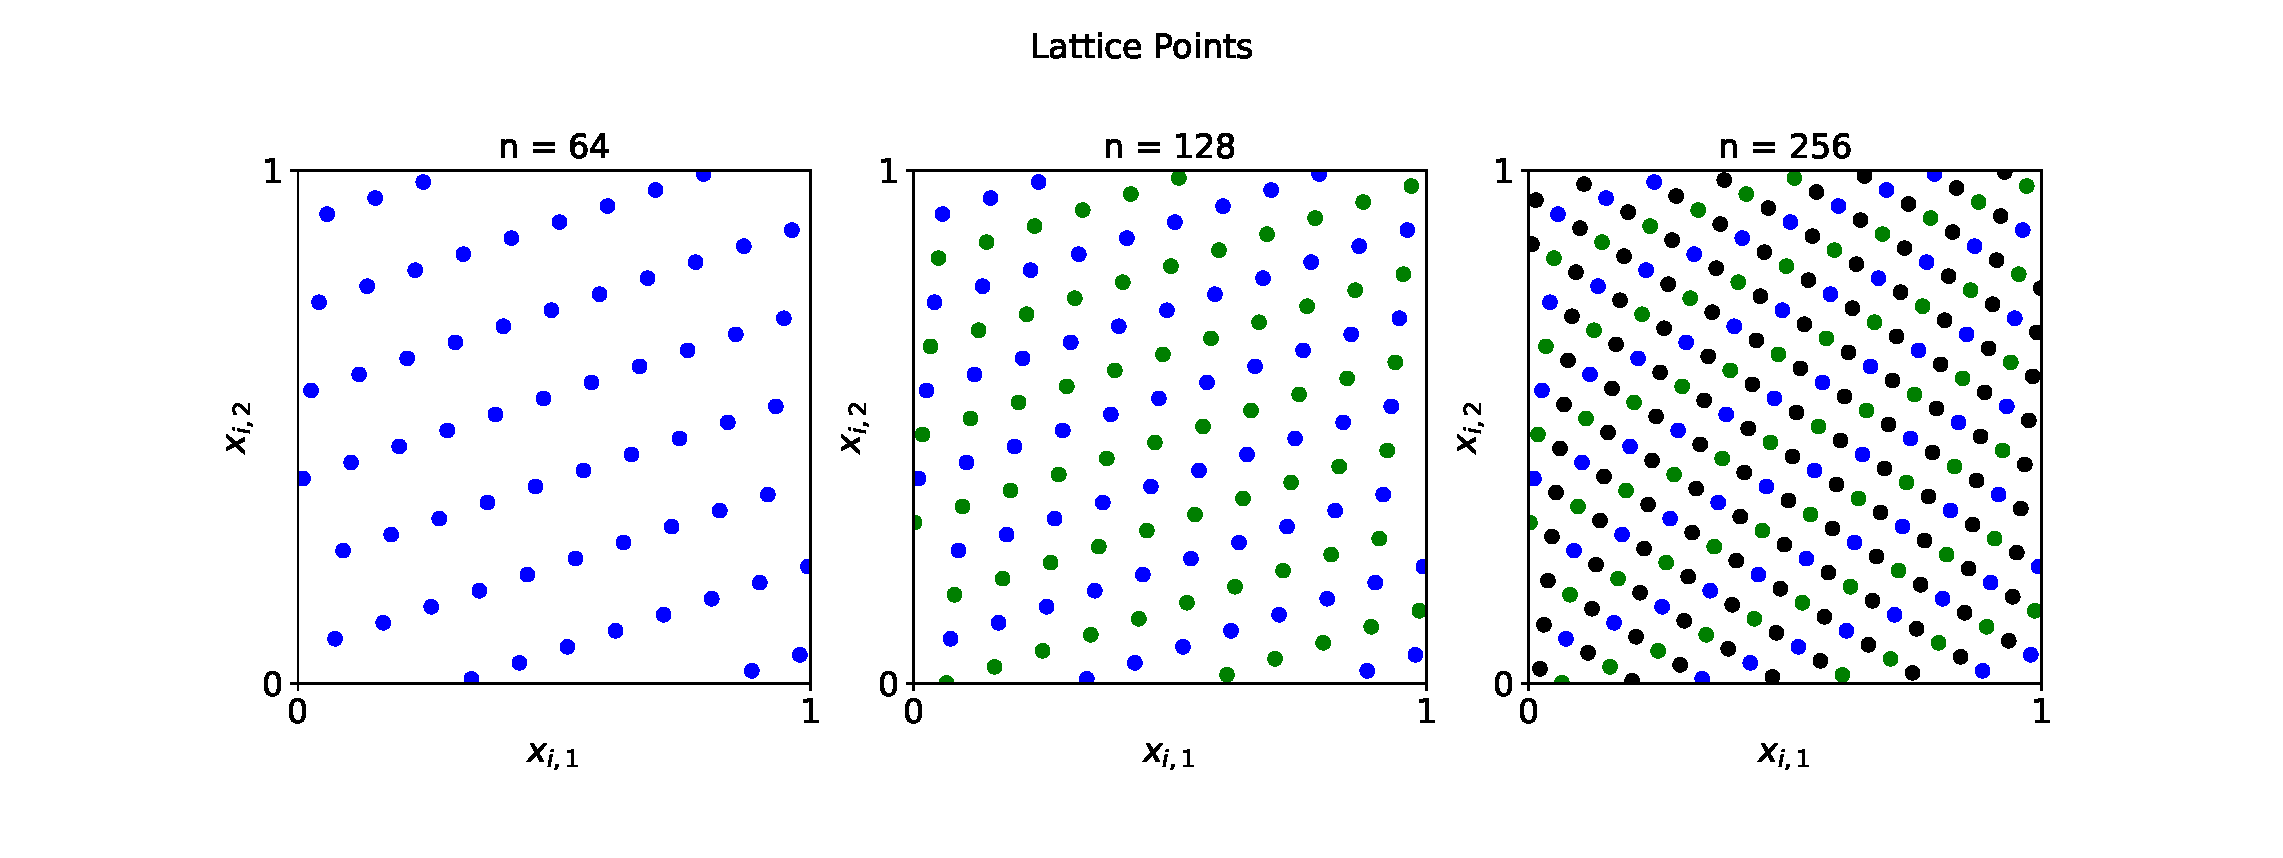
\includegraphics[width = \textwidth]{figures/dd_Lattice.eps}
	
	\vspace{-7ex}
\[
C_\vtheta(\vt,\vx) = K_\vtheta(\vt - \vx \bmod \vone), \qquad \text{e.g., }K_\vtheta(\vt) = \prod_{k=1}^d\bigl[ 1  +  \eta_k  (-1)^{r+1} \underbrace{B_{2r}(t_k)}_{\substack{\text{Bernoulli}\\ \text{polynomial}}} \bigr], \quad \vtheta = (r,\veta)
\]	
}
\only<3>{LD digital sequences \cite{Nie92,DicPil10a,DicEtal14a} (e.g., Sobol') are more even than IID  and give faster convergence
	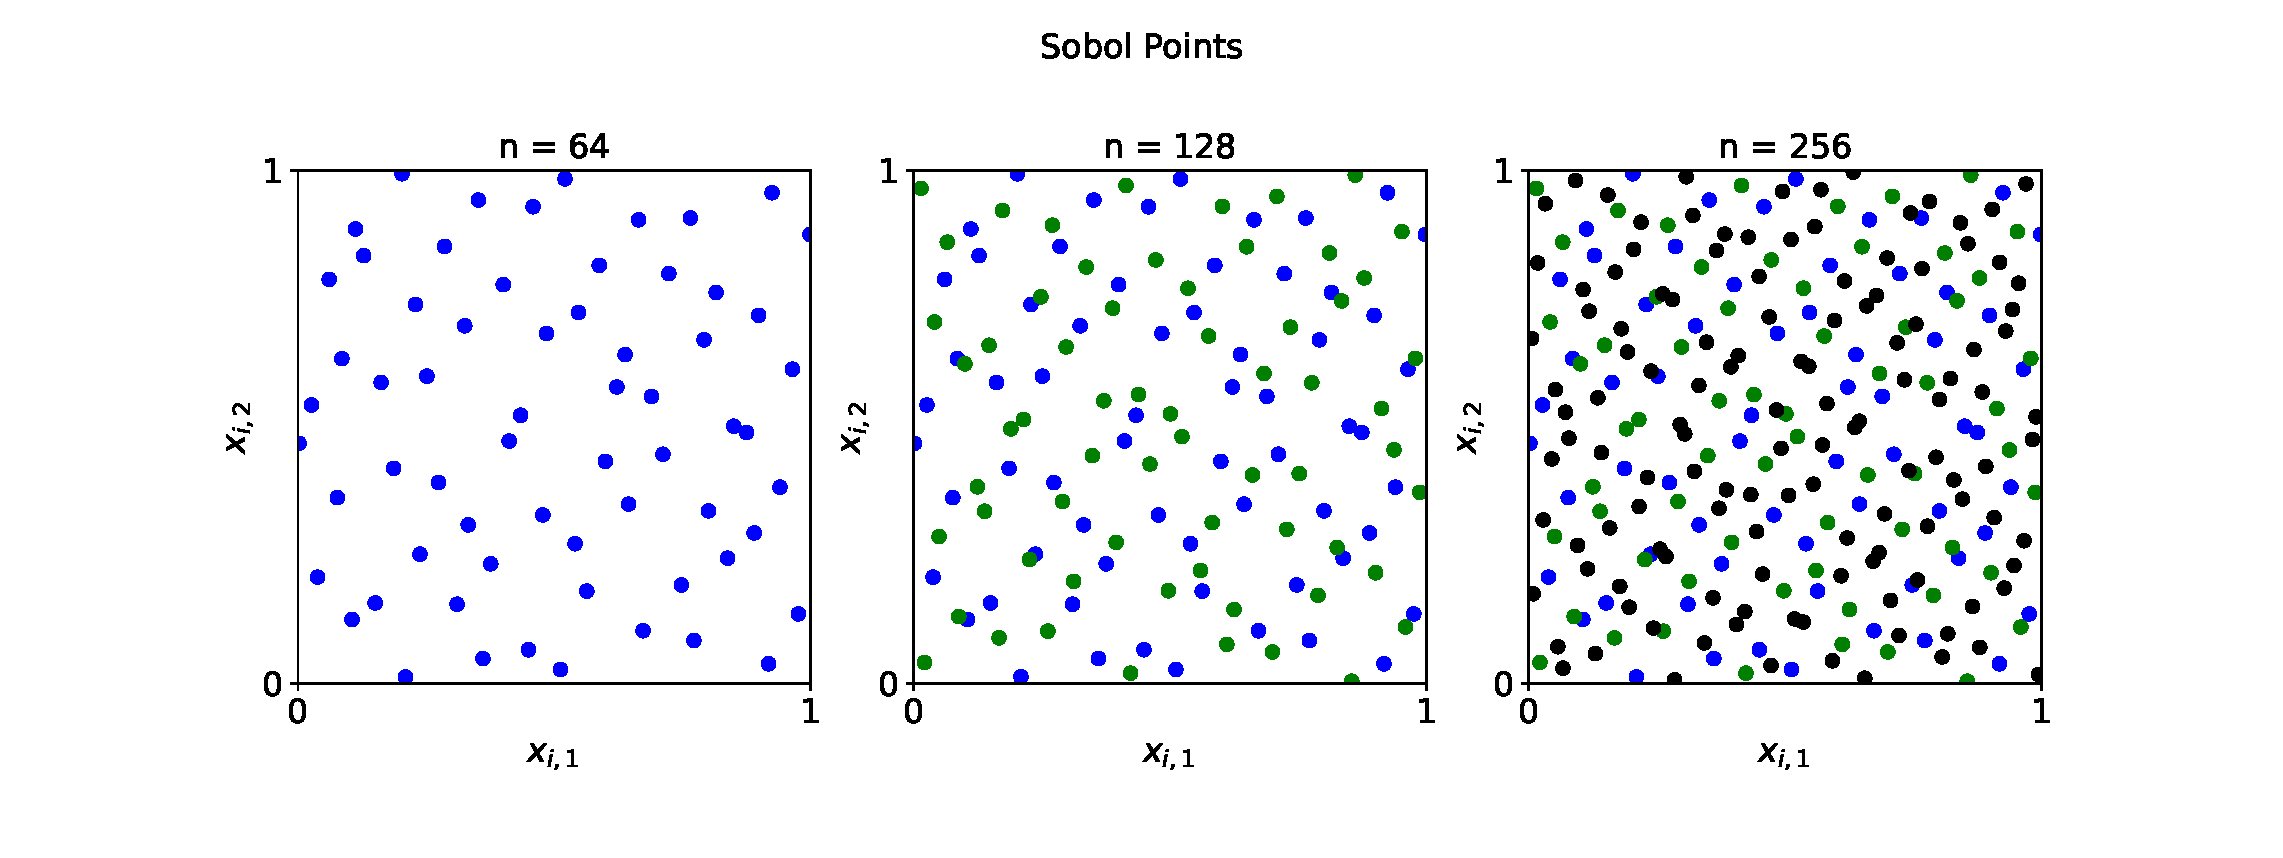
\includegraphics[width = \textwidth]{figures/dd_Sobol.eps}
	
	\vspace{-7ex}
	\[
	C_\vtheta(\vt,\vx) = K_\vtheta(\vt \underbrace{\ominus}_{\substack{\text{digitwise}\\ \text{subtraction}}} \vx ), \qquad \text{e.g., }K_\vtheta(\vt) = \prod_{k=1}^d\bigl[ 1+ \eta_k \underbrace{\omega(t_k)}_{\text{explicit}}\bigr], \quad \vtheta = (r,\veta)
	\]	
}

\end{frame}

\begin{frame}{\only<1>{Eigenvector-Eigenvalue Decomposition of the Gram Matrix}\only<2->{Tuning Hyperparameters in $\GP(m,s^2 C_\vtheta)$ and the Credible Interval} \cite{HicJag18b,RatHic19a,Jag19a,JagHic22a}}
	For these matched data sites and covariance kernels
	\begin{gather*}
		\only<1-2>{\int_{[0,1]^d} C_\vtheta(\vt,\vx) \, \dif \vt = 1 \quad \forall \vx \in [0,1]^d, \qquad
		\mC_\vtheta = \bigl(C_\vtheta(\vx_i, \vx_j)\bigr)_{i,j=1}^n= \bigl( \vC_{\vtheta 1}, \ldots, \vC_{\vtheta n}) =\frac 1n  \mV \mLambda_\vtheta \mV^H\\
	  \mV \text{ \alert{explict} (complex exponential/Hadamard)}, \qquad \vV_1 = \vone \\}
	  \vb \mapsto \tvb := \mV^H \vb \text{ is \alert{FFT/FHWT} } \Order (n \log n), \qquad \vlambda_\vtheta := \diag(\mLambda_\vtheta) = \mV^H \vC_{\vtheta 1} = \widetilde{\vC}_{\vtheta 1}
	\end{gather*} 
\uncover<2->{which leads to the approximation and credible interval:
\begin{gather*}
	\hmu = \frac{\ty_1}{n} = \frac 1n \sum_{i=1}^n f(\vx_i) = \text{sample mean}, \qquad \vy = \bigl(f(\vx_1), \ldots, f(\vx_n) \bigr)^T, \quad \tvy = \mV^H \vy\\
\Prob \bigl [\abs{\mu - \hmu} \le \ERR\bigr ] = 99\%,  \qquad 
\ERR = \frac{2.58}{n} \sqrt{ \sum_{i = \alert{2}}^n \frac{\lvert \ty_i \rvert^2}{\lambda_{\vtheta i}} \left(1 - \frac{n}{\lambda_{\vtheta 1}} \right)} 
\only<3>{ \\
\vtheta_{\text{opt}} =  \argmin_{\vtheta} \left [ \log \left( \sum_{i=\alert{2}} \frac{\lvert \ty_i \rvert^2}{\lambda_{\vtheta i}}\right)   + \frac 1n \sum_{i=1}^n \log(\lambda_{\vtheta i} )  \right ]
}
\end{gather*}
}

\end{frame}
	
\section{QMCPy}

\begin{frame}{Our Bayesian Stopping Criteria into Software}
	
	\vspace{-3ex}
	
	Our research on stopping criteria (Bayesian and otherwise) has been implemented in
	\begin{itemize}
		\item GAIL \cite{ChoEtal21a} MATLAB library (born in 2013)
		\item QMCPy \cite{QMCPy2020a} Python library (born in 2019)
	\end{itemize}
We aim to provide software that 
\begin{itemize}
	\item Includes the best---mostly quasi-Monte Carlo (QMC)---algorithms available
	\item Is well-tested
	\item Is an easy on-ramp for practitioners
	\item Provides use cases for algorithm developers 
	\item Plays well with other packages
\end{itemize}
	
	
\end{frame}
	

\begin{frame}[fragile]\frametitle{Keister Example in QMCPy \href{https://colab.research.google.com/drive/1KrlrtLu7j8Ff7YsSJjPMiGUr-UKfqwxm?usp=sharing}{\beamergotobutton{computations in Google colab notebook here}}}
	\vspace{-5ex}
	\[
	\mu = \int_{\reals^d} \cos(\norm{\vt}) \exp(-\norm{\vt}^2) \, \dif \vt = \int_{[0,1]^d} f(\vx) \; \dif \vx =  ? \qquad \text{Keister \cite{Kei96}}
	\]
\noindent\begin{minipage}{0.47\textwidth}
\begin{lstlisting}[style=Python]
d = 5; tol = 1e-2
lattice = Lattice(dimension = d, order = 'linear')
integrand = Keister(lattice)
stop_crit = CubBayesLatticeG(integrand, abs_tol = tol, ptransform = 'none')
solution,data = stop_crit.integrate()
print(data)
\end{lstlisting}
\end{minipage} 
\qquad
\begin{minipage}{0.47\textwidth}
\begin{lstlisting}[style=Python]
solution        1.136
error_bound     0.009
n_total         1024
time_integrate  0.725
abs_tol         0.010
rel_tol         0
n_init          2^(8)
n_max           2^(22)
\end{lstlisting}
\end{minipage} 

\end{frame}


\begin{frame}[fragile]\frametitle{Asian Option Pricing Example in QMCPy \href{https://colab.research.google.com/drive/1KrlrtLu7j8Ff7YsSJjPMiGUr-UKfqwxm?usp=sharing}{\beamergotobutton{computations here}}}
	\vspace{-5ex}
	\[
	\text{option price} = \mu = \int_{\reals^d} \text{payoff}(\vz) \; \text{discrete BM PDF}(\vz)   \, \dif \vz = \int_{[0,1]^d} f(\vx) \; \dif \vx  = ? \quad \text{Glasserman  \cite{Gla03}}
	\]
\noindent\begin{minipage}{0.52\textwidth}
\begin{lstlisting}[style=Python]
volatility=.5; interest_rate =.01
start_price = 30; strike_price = 25
t_final = 1; call_put = 'call'
mean_type = 'arithmetic'
d = 4; abs_tol = .01
integrand = AsianOption(Lattice(d, order = 'linear'), volatility, start_price, strike_price, interest_rate, t_final, call_put, mean_type)
solution,data = CubBayesLatticeG(integrand, abs_tol = abs_tol).integrate()
print(data)
\end{lstlisting}
\end{minipage} 
\qquad
\begin{minipage}{0.42\textwidth}
\begin{lstlisting}[style=Python]
solution        6.235
error_bound     0.007
n_total         2048
time_integrate  1.470
abs_tol         0.010
rel_tol         0
time_vec        [0.25 0.5  0.75 1.  ]
covariance      [[0.25 0.25 0.25 0.25]
[0.25 0.5  0.5  0.5 ]
[0.25 0.5  0.75 0.75]
[0.25 0.5  0.75 1.  ]]
decomp_type     PCA
\end{lstlisting}
\end{minipage} 
	
\end{frame}


\section{Challenges}

\begin{frame}\frametitle{Slow Speed, Wrong Answers \href{https://colab.research.google.com/drive/1KrlrtLu7j8Ff7YsSJjPMiGUr-UKfqwxm?usp=sharing}{\beamergotobutton{computations here}}}
{\small 
\vspace{-3ex}
\begin{center}
\begin{tabular}{rccccl}
	Example & Stopping Criterion & $d$ & Absolute Tolerance & $n$ & Time \\ \toprule
	Keister & Bayesian Lattice \cite{RatHic19a} & $5$ & $0.01$ & $2^{10}$ & $0.725$ s \\
	Keister & Bayesian Sobol' \cite{JagHic22a} &&&  $2^{12}$ & $0.102$ s \\
	Keister & Track Fourier Coef.\ Lattice \cite{JimHic16a} &&& $2^{13}$ & $0.024$ s \\
	Keister & Track Fourier Coef.\  Sobol' \cite{HicJim16a} &&& $2^{13}$ & $0.012$ s \\ \midrule
	Keister & Bayesian Lattice \cite{RatHic19a} & $5$ & $0.001$ &  & \alert{$> 10$ m} \\
	Keister & Track Fourier Coef.\ Lattice \cite{JimHic16a} &&& $2^{17}$ & $0.388$ s \\ \toprule
Option Pricing  & Bayesian Lattice \cite{RatHic19a} & $4$ & $0.01$ & $2^{11}$ & $1.470$ s \\
Option Pricing  & Track Fourier Coef.\ Lattice \cite{JimHic16a} &&& $2^{12}$ & $0.021$ s \\ \midrule
Option Pricing  & Bayesian Lattice \cite{RatHic19a} & $13$ & $0.01$ & \multicolumn{2}{c}{\alert{wrong answer}}\\
Option Pricing  & Track Fourier Coef.\ Lattice \cite{JimHic16a} &&& $2^{12}$ & $0.034$ s \\ \bottomrule
\end{tabular}
\end{center}
\vspace{-3ex}
\begin{itemize}
	\setlength{\itemsep}{-0.5ex}
	\item Computational load in \alert{optimizing} for the kernel parameters
	\item \alert{Inefficient} code
	\item Speed may not be a problem if function evaluation is \alert{expensive}
\end{itemize}
}
\end{frame}

\begin{frame}[fragile]\frametitle{Checking the Gaussian Process Assumption}

\vspace{-3ex}
If $\bigl(f(\vx_1), \ldots, f(\vx_n)\bigr) ^T$ has a known multivariate Gaussian distribution, then the correct transformation of this data has a standard univariate Gaussian distribution

Here are QQ plots for the Keister example with different randomized lattice data sites and $n=64$

\centerline{%
    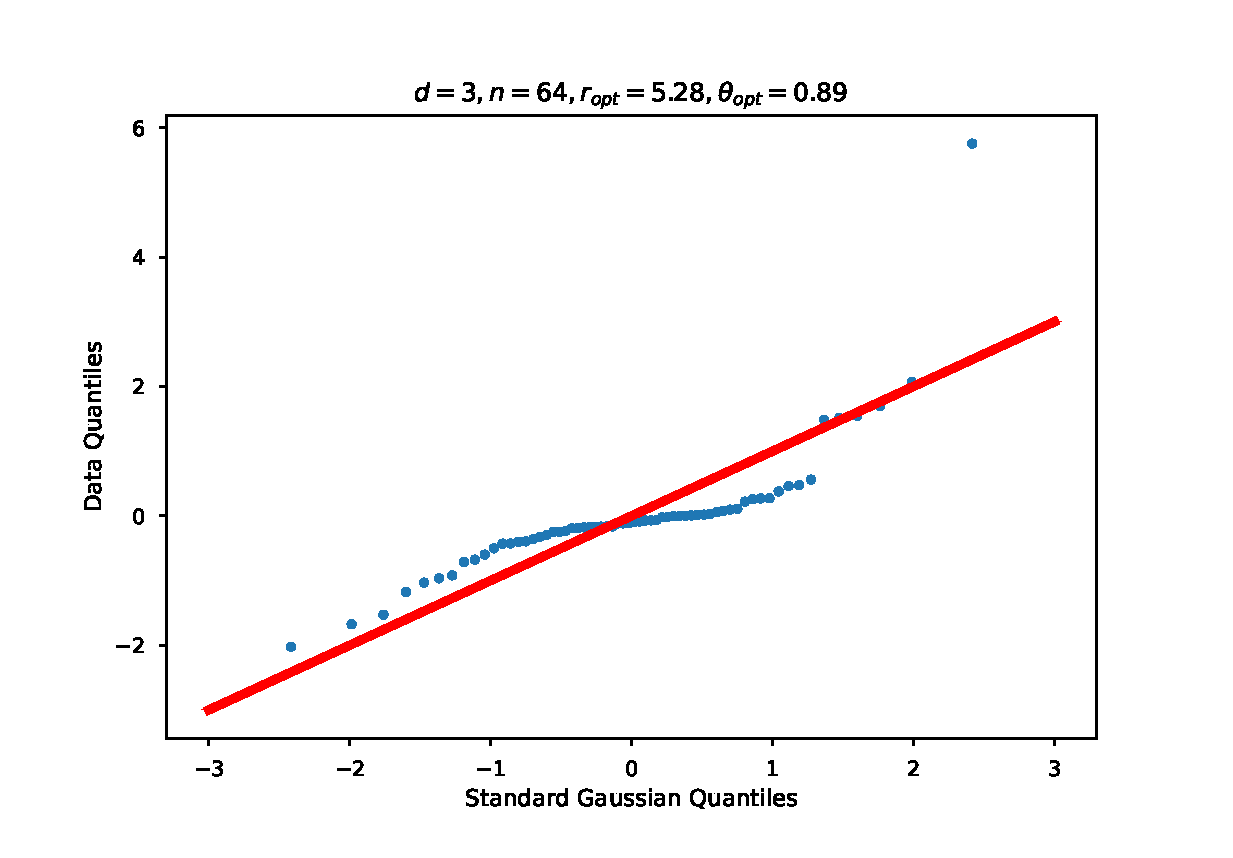
\includegraphics[width=0.35\textwidth]{figures/Keister-QQPlot_n-64_d-3_case-7.eps} \hspace{-3ex}
	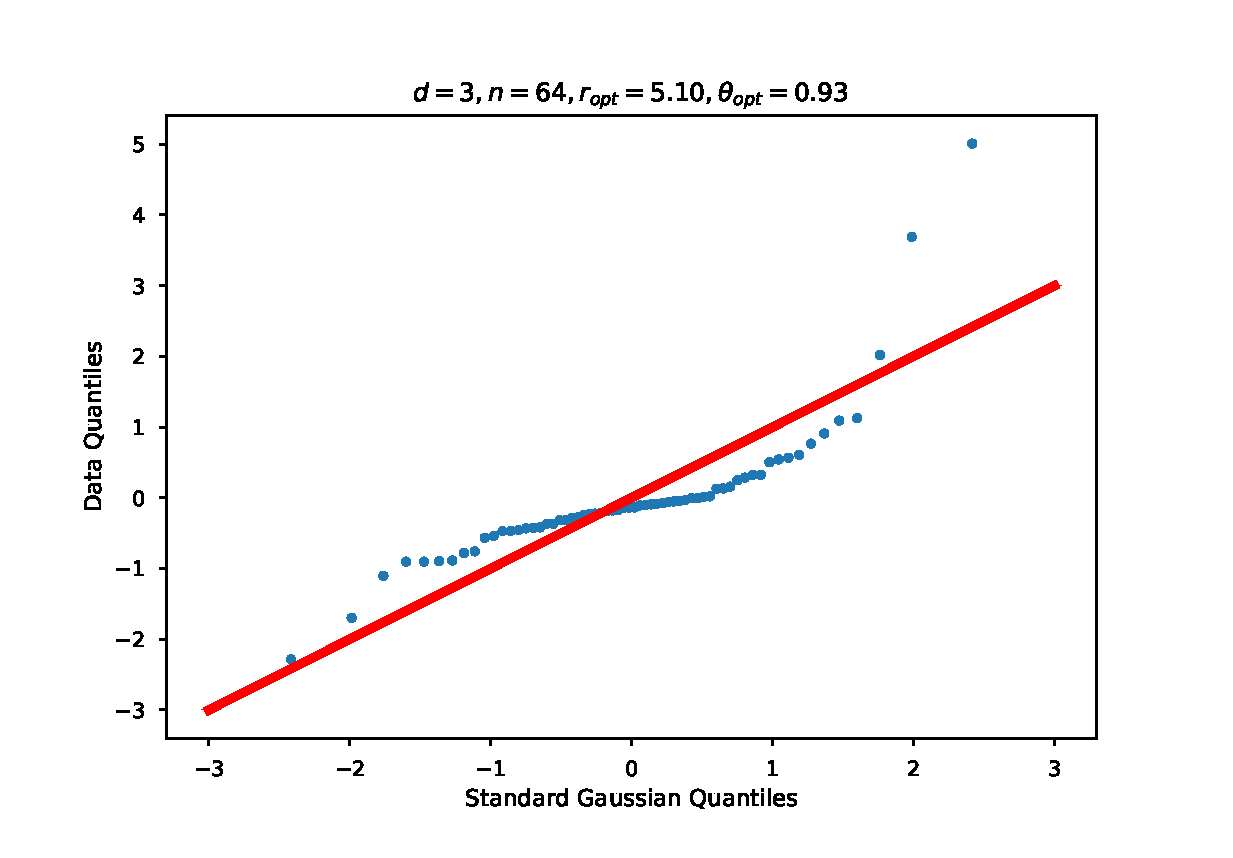
\includegraphics[width=0.35\textwidth]{figures/Keister-QQPlot_n-64_d-3_case-1.eps} \hspace{-3ex}
	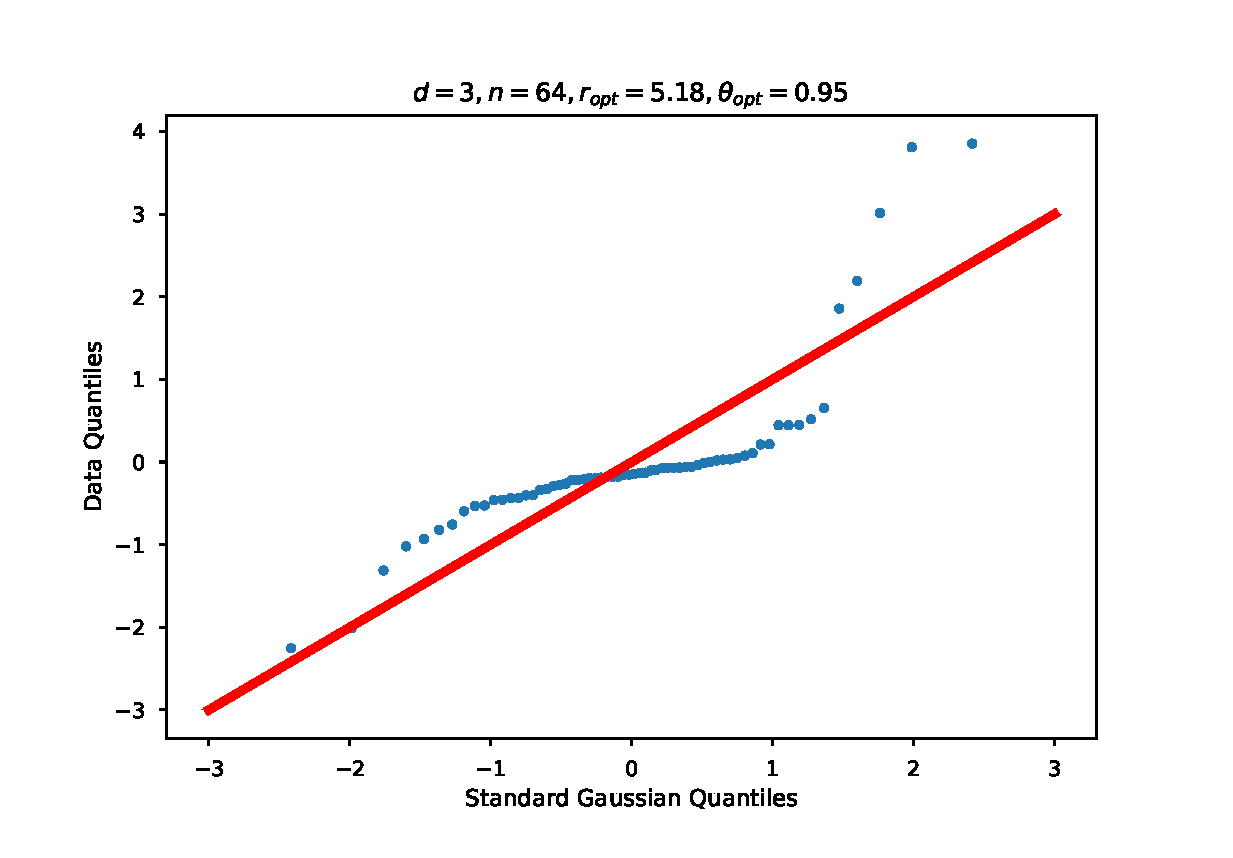
\includegraphics[width=0.35\textwidth]{figures/Keister-QQPlot_n-64_d-3_case-2.eps}}

Should we be concerned?

\end{frame}



\section{Summary}
\begin{frame}\frametitle{Summary}
	
\vspace{-5ex}
	
\begin{itemize}
	\item Bayesian cubature using credible intervals as stopping criteria often gives correct answers
	
	\item Matching sampling sites (designs) with covariance kernels expedites the computation
	
	\item Tuning the hyperparameters can add significant computational load
	
	\item Challenges of speeding up the computation and finding the right kernels or hyperparameters still remain
\end{itemize}
	
\end{frame}



\finalthanksnote{These slides are  available at \\  \href{https://speakerdeck.com/fjhickernell/dagstuhl-bayesian-cubature-ld-qmcpy}{\nolinkurl{speakerdeck.com/fjhickernell/dagstuhl-bayesian-cubature-ld-qmcpy}}}


\thankyouframe

\begin{frame}[allowframebreaks]{References}
\printbibliography
\end{frame}
	
\end{document}



